% !TEX encoding = UTF-8
% !TEX TS-program = pdflatex
% !TEX root = ../tesi.tex

%**************************************************************
\chapter{Svolgimento dello stage}
\label{cap:svolgimento-dello-stage}
%**************************************************************

%\intro{Breve introduzione al capitolo}\\

%**************************************************************
\section{Pianificazione}

Il Piano di Lavoro, redatto insieme al tutor aziendale, prevedeva inizialmente 4 fasi, ognuna delle quali della durata di 3 settimane lavorative:
\begin{itemize}
	\item studio del processo aziendale e formazione sulle tecnologie coinvolte nello sviluppo della \textit{webapp} e dell'interfacciamento con il gestionale;
	\item progettazione della soluzione e configurazione dell'ambiente di sviluppo;
	\item realizzazione della \textit{webapp} e fase di \textit{testing};
	\item formazione sul software per la produzione di stampe e sviluppo dei report;
\end{itemize}
L'ultima settimana di stage prevedeva la verifica e validazione finale.
Di seguito un dettaglio delle fasi appena descritte:

\begin{center}
	\begin{longtable}{|c|c|}
		\caption{Dettaglio pianificazione del progetto di stage.}\\		
		\hline
		\textbf{Ore} & \textbf{Attività}\\
		\hline
		40 & Formazione sulle tecnologie\\
		\hline
		35 & Analisi del problema\\
		\hline
		25 & Stesura documentazione relativa ad analisi e progettazione\\
		\hline
		55 & Progettazione della soluzione\\
		\hline
		15 & Configurazione dell'ambiente di sviluppo\\
		\hline
		60 & Sviluppo dell'applicazione web\\
		\hline
		20 & Test su applicazione web\\
		\hline
		25 & Test su \textit{web services}\\
		\hline
		25 & Formazione su strumento e produzione report\\
		\hline
		5 & Stesura documentazione finale\\
		\hline
		15 & Verifica e validazione finale\\
		\hline
	\end{longtable}
\end{center}


Nella sezione successiva sono descritte le problematiche riscontrate che hanno portato alla modifica della pianificazione appena mostrata.
\newpage

%**************************************************************


\section{Analisi dei requisiti}

\subsection{Processo aziendale}

Attualmente vengono gestite due tipologie di richieste di offerta:
\begin{itemize}
	\item acquisto di beni e servizi;
	\item richieste di trasporto merci.
\end{itemize}
Le richieste di acquisto di beni e servizi (come servizi di pulizia, di vigilanza ecc.) vengono ad oggi interamente gestite all'interno del gestionale. 
Le richieste di trasporto merci, invece, vengono effettuate attraverso la compilazione di un modulo cartaceo (chiamato MPQ), contenente tutte le caratteristiche dell'offerta; il modulo è veicolato tra i diversi uffici che ne compilano le sezioni di competenza:
\begin{itemize}
	\item \textbf{ufficio Commerciale}, che inserisce i dati necessari alla consegna;
	\item \textbf{ufficio Logistica}, che inserisce le informazioni sul carico e il trasporto;
	\item \textbf{ufficio Acquisti}, che perviene il modulo compilato e lo invia ai fornitori designati.
\end{itemize}
Una volta ricevute le risposte, l'ufficio acquisti designa il vincitore e lo comunica all'ufficio commerciale, che contatta il cliente per l'accettazione o il rifiuto dell'offerta.


\subsection{Problematiche attuali}
Le comunicazioni tra uffici e fornitori sono effettuate telefonicamente o via e-mail e non vi è traccia all'interno del gestionale di alcun dato (numero di richieste effettuate, numero di richieste accettate/respinte, ecc) ad eccezione del prezzo dell'offerta del fornitore vincitore della gara, che viene inserito manualmente dall'ufficio acquisti.
La soluzione proposta inizialmente dall'azienda, ovvero la creazione di un'applicazione web utilizzabile sia dagli utenti che dai fornitori, non sarebbe andata incontro pienamente alle esigenze degli utenti: infatti quest'ultimi avrebbero dovuto utilizzare un'applicazione esterna all'ambiente del gestionale. 
Questo avrebbe comportato:
\begin{itemize}
	\item ulteriore formazione per gli utenti;
	\item spostamento tra ambienti diversi (gestionale e applicazione web), perdita di tempo nel passaggio dall'uno all'altra rispetto all'utilizzo del solo gestionale.
\end{itemize}
Oltre a questo, il nuovo gestionale Sage X3 presenta una funzionalità di gestione delle richieste di offerta di default, fortemente personalizzabile.
Ecco quindi, che in accordo con il tutor aziendale, ho quindi ridefinito la soluzione rispetto a quella inizialmente proposta dall'azienda.

\subsection{Soluzione proposta}
Vista la funzionalità offerta da Sage X3 e i limiti della prima soluzione proposta dall'azienda, ho ritenuto opportuno ridefinire la soluzione personalizzando all'interno di Sage X3 il modulo di gestione delle richieste di offerta, che verrà utilizzato dagli utenti interni.
L'applicazione web, che sarà pertanto utilizzata solo dai fornitori per rispondere alle richieste di offerta, comunicherà con il gestionale tramite \textit{web services} SOAP.
Questa modifica ha richiesto un aggiornamento delle attività e della pianificazione dello stage, come segue:

\begin{center}
	\begin{longtable}{ | c| c|}
		\caption{Dettaglio pianificazione aggiornata del progetto di stage.}\\	
		\hline
		\textbf{Ore} & \textbf{Attività}\\
		\hline
		55 & Formazione sulle tecnologie\\
		\hline
		35 & Analisi del problema\\
		\hline
		25 & Stesura documentazione relativa ad analisi e progettazione\\
		\hline
		55 & Progettazione della soluzione\\
		\hline
		15 & Configurazione dell'ambiente di sviluppo\\
		\hline
		20 & Sviluppo dell'interfaccia nel gestionale\\
		\hline
		5 & Test su interfaccia gestionale\\
		\hline
		35 & Sviluppo dell'applicazione web\\
		\hline
		15 & Test su applicazione web\\
		\hline
		15 & Test su \textit{web services}\\
		\hline
		25 & Formazione su strumento e produzione report\\
		\hline
		5 & Stesura documentazione finale\\
		\hline
		15 & Verifica e validazione finale\\
		\hline
	\end{longtable}
\end{center}

\begin{figure}[htbp]
	\begin{center}
		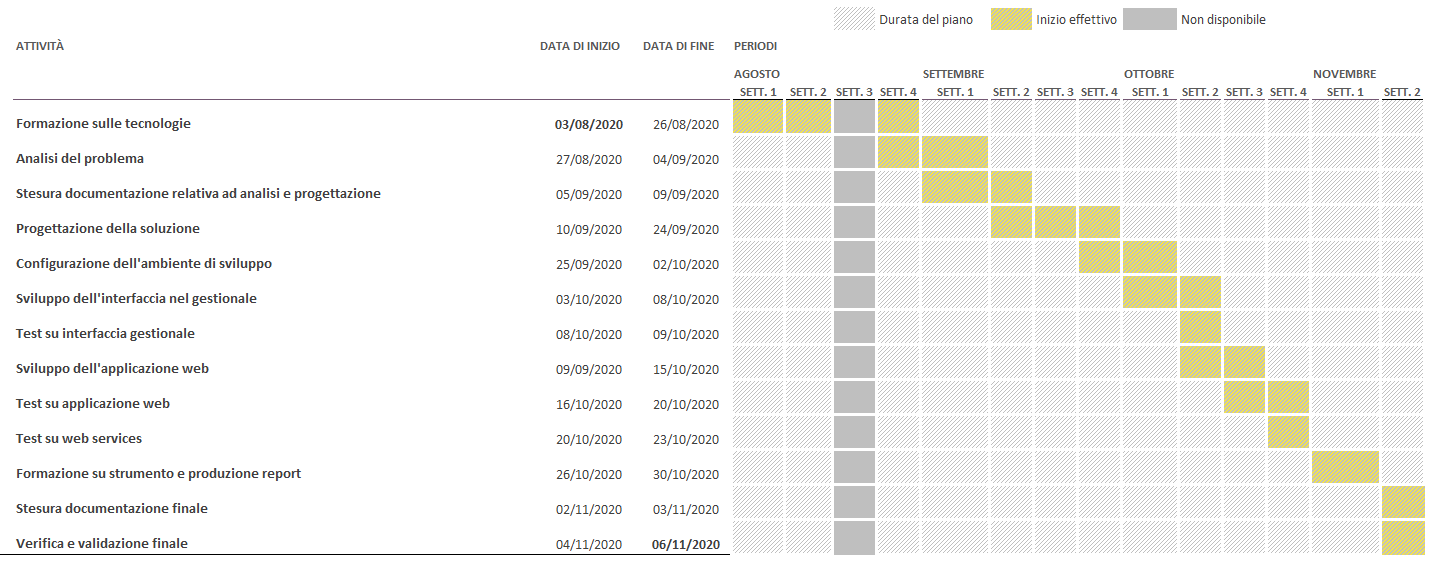
\includegraphics[height=5.5cm]{gantt}
		\caption{Rappresentazione della pianificazione con diagramma di Gantt.}
	\end{center}
\end{figure}

Come si evince dal dettaglio, sono aumentate le ore dedicate alla formazione, per apprendere le nozioni fondamentali necessarie a sviluppare l'interfaccia nel gestionale. Sono diminuite le ore necessarie allo sviluppo dell'applicazione web, in quanto la gestione delle richieste da parte degli utenti aziendali viene fatta all'interno di Sage X3 e sono state aggiunte le ore necessarie all'implementazione e ai test dell'interfaccia del gestionale.

\subsection{Requisiti}
I requisiti che ho individuato sono stati classificati, assieme al tutor aziendale, per tipologia:
\begin{itemize}
	\item \textbf{funzionali}, che individuano tutte le funzionalità previste dall'applicazione web e dall'interfaccia in Sage X3;
	\item \textbf{qualitativi}, in cui ho inserito l'utilizzo del sistema di versionamento con Github;
	\item \textbf{di vincolo}, in cui rientrano i vincoli sulle tecnologie da utilizzare nello sviluppo del progetto, ossia \textit{framework} e \textit{web services}; 
	\item \textbf{prestazionali}, non è risultato necessario definire alcun vincolo necessario a garantire alcuna prestazione.
\end{itemize}
Oltre alla tipologia, i requisiti vengono suddivisi anche per importanza:
\begin{itemize}
	\item \textbf{obbligatori}, necessari alla realizzazione del progetto;
	\item \textbf{desiderabili}, non necessari ma se soddisfatti portano valore aggiunto al prodotto.
\end{itemize}


\begin{center}
\begin{longtable}{ | c| c | c | c|}
	\caption{Tabella di riepilogo requisiti.}\\
	\hline
	\textbf{Tipo} & \textbf{Obbligatorio} & \textbf{Desiderabile} & \textbf{Totale}\\
	\hline
	\textbf{Funzionale} & 25 & 1 & 26 \\
	\hline
	\textbf{Qualitativo} & 1 & 0 & 1\\
	\hline
	\textbf{Vincolo} & 3 & 0 & 3 \\
	\hline
	\textbf{Prestazionale} & 0 & 0 & 0 \\
	\hline
	\textbf{Totale} & 29 & 1 & 30 \\
	\hline
\end{longtable}
\end{center}


\begin{figure}[htbp]
	\begin{center}
		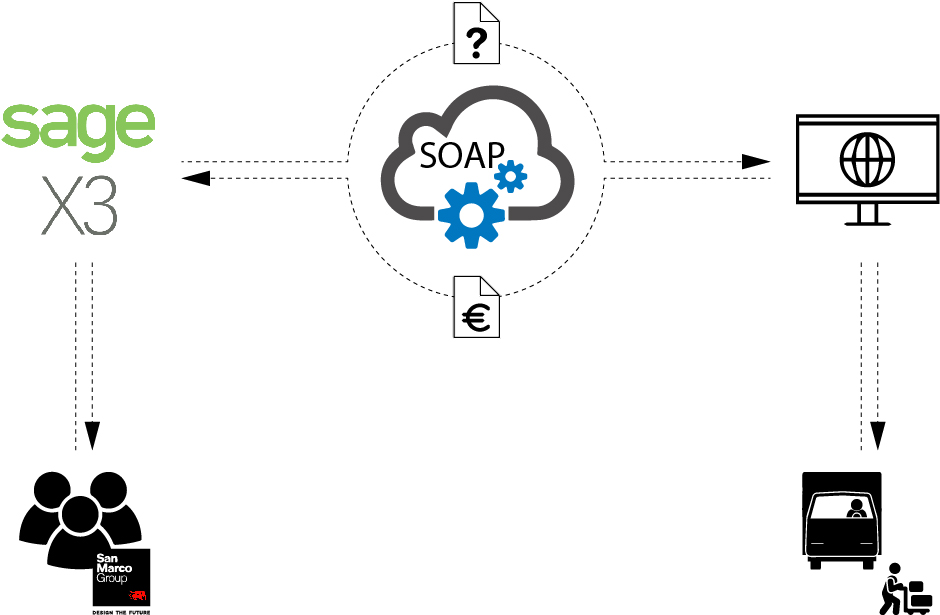
\includegraphics[height=6.5cm]{soluzione}
		\caption{Architettura della soluzione realizzata.}
	\end{center}
\end{figure}


%**************************************************************


\section{Progettazione e codifica}

\subsection{Tecnologie e strumenti utilizzati}

\paragraph{Visual Studio}
Visual Studio nella sua versione 2019 è l'IDE che ho utilizzato come ambiente di sviluppo per la creazione dell'applicazione web. L'IDE incorpora la versione 4.7.2 di .NET Framework, ambiente di esecuzione \textit{runtime} della piattaforma tecnologica .NET.
Ho scelto questo strumento in primo luogo perché è l'ambiente utilizzato maggiormente all'interno dell'azienda, per la sua compatibilità ed estendibilità con i vari applicativi e servizi Microsoft presenti nell'infrastruttura interna. Inoltre dispone di un \textit{debugger} interno che ho utilizzato per verificare e testare i vari metodi realizzati.

\paragraph{Bootstrap}
Bootstrap è un framework \textit{front-end} gratuito e open source per la progettazione di
siti e applicazioni web. Contiene modelli di progettazione basati su HTML e
CSS per moduli, pulsanti, navigazione e altri componenti dell'interfaccia, nonché
estensioni JavaScript facoltative. Per realizzare l'interfaccia dell'applicazione web ho sfruttato il tema gratuito e open source \textit{SB admin 2}, messo a disposizione dal framework.

\paragraph{SQL Server}
\textit{SQL Server} è un \textit{DBMS} (\textit{Database Management System}) relazionale sviluppato da \textit{Microsoft}. Viene utilizzato per gestire database delle dimensioni e strutture più disparate.
Per interagire e manipolare i dati in \textit{SQL Server}, ho utilizzato \textit{SQL Server Management Studio}, un programma sviluppato appositamente da \textit{Microsoft} il cui utilizzo è già adottato e consolidato in azienda.

\paragraph{Git}
Il sistema di \textit{versioning} adottato per questo progetto e in generale utilizzato dall'azienda è Git.
L'azienda adotta attualmente GitHub, un servizio di hosting per progetti basato su Git.
Ho utilizzato GitKraken, un client \textit{GUI} (\textit{Graphic User Interface}) per rendere più facile e veloce l'utilizzo del sistema di versionamento.

\begin{figure}[htbp]
	\begin{center}
		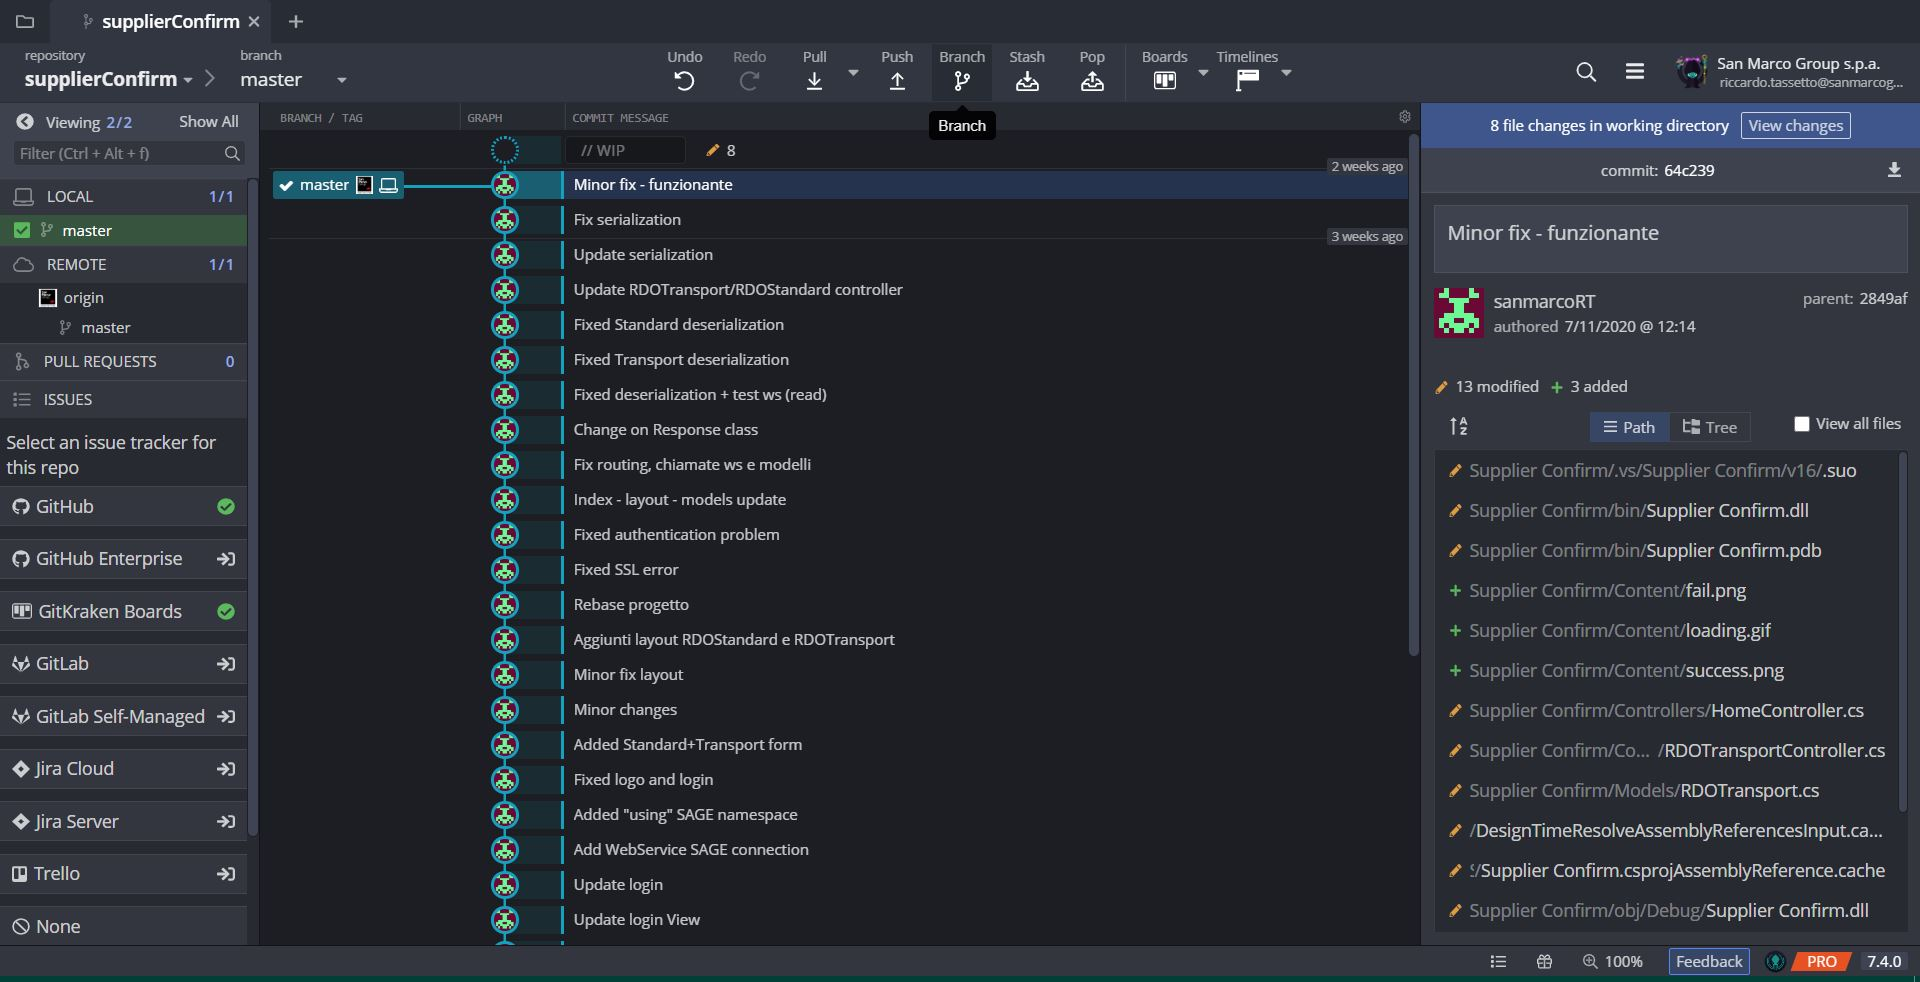
\includegraphics[height=6cm]{gitkraken}
		\caption{Schermata che mostra il repository del progetto su Gitkraken.}
	\end{center}
\end{figure}


\paragraph{Tecnologia SOAP}
\textit{SOAP} (\textit{simple object access protocol}) è un protocollo che regola lo scambio di messaggi tra componenti software. Opera principalmente sul protocollo di rete \textit{HTTP}, si basa sul metalinguaggio \textit{XML} e ha una struttura costituita da:
\begin{itemize}
	\item \textit{\textbf{header}}, che contiene le informazioni necessarie per l'instradamento e la sicurezza; 
	\item \textit{\textbf{body}}, che contiene i dati formattati secondo l'XML Schema.
\end{itemize}


%*********************************************************************************


\subsection{Interfaccia del gestionale}
Una volta appreso le nozioni basilari attraverso la documentazione disponibile e tramite un affiancamento con i fornitori del gestionale per conoscere la funzionalità già
presente, ho sviluppato l'interfaccia che verrà utilizzata dagli utenti per la gestione delle richieste di offerta.

\subsubsection{Introduzione a Sage X3}
Sage X3 è un ERP sviluppato utilizzando un linguaggio proprietario.
La gestione degli oggetti X3 è alla base della maggior parte delle funzioni messe a disposizione dal software.
Un oggetto X3 corrisponde alla gestione completa delle schede di una tabella o di un gruppo di tabelle del database (creazione, consultazione, modifica e annullamento).
Ad esempio, la funzionalità di gestione delle richieste di offerta è stata implementata nel software gestionale utilizzando un oggetto X3, denominato \textit{PQH}.

\begin{figure}[htbp]
	\begin{center}
		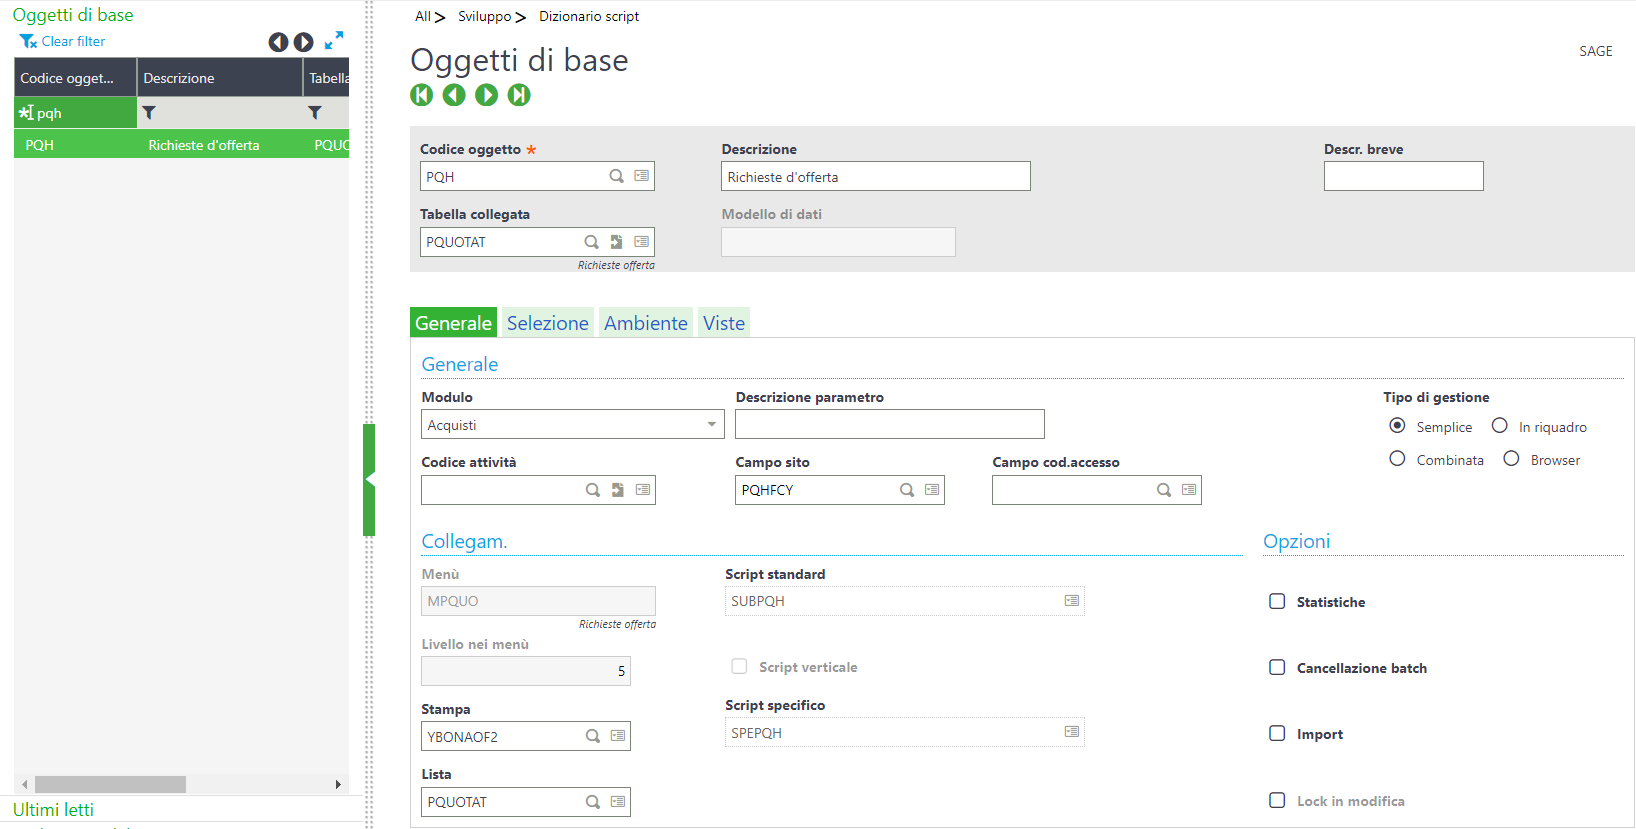
\includegraphics[height=6cm]{oggettoX3}
		\caption{Schermata che mostra la rappresentazione di un oggetto X3.}
	\end{center}
\end{figure}

\newpage

L'oggetto PQH si presenta come una finestra composta da una testata, da più blocchi (ovvero campi che contengono riferimenti ad altri oggetti X3), dai campi che corrispondo ai suoi attributi e da una lista di selezione situata a sinistra chiamata \textit{browser}. Il \textit{browser} permette una ricerca parametrizzata di una specifica istanza di quell'oggetto. Il menù presente sulla destra invece mostra le operazioni messe a disposizione dalla funzionalità, suddivise per \textit{folder}, ovvero dei raggruppamenti di operazioni affini.

\begin{figure}[htbp]
	\begin{center}
		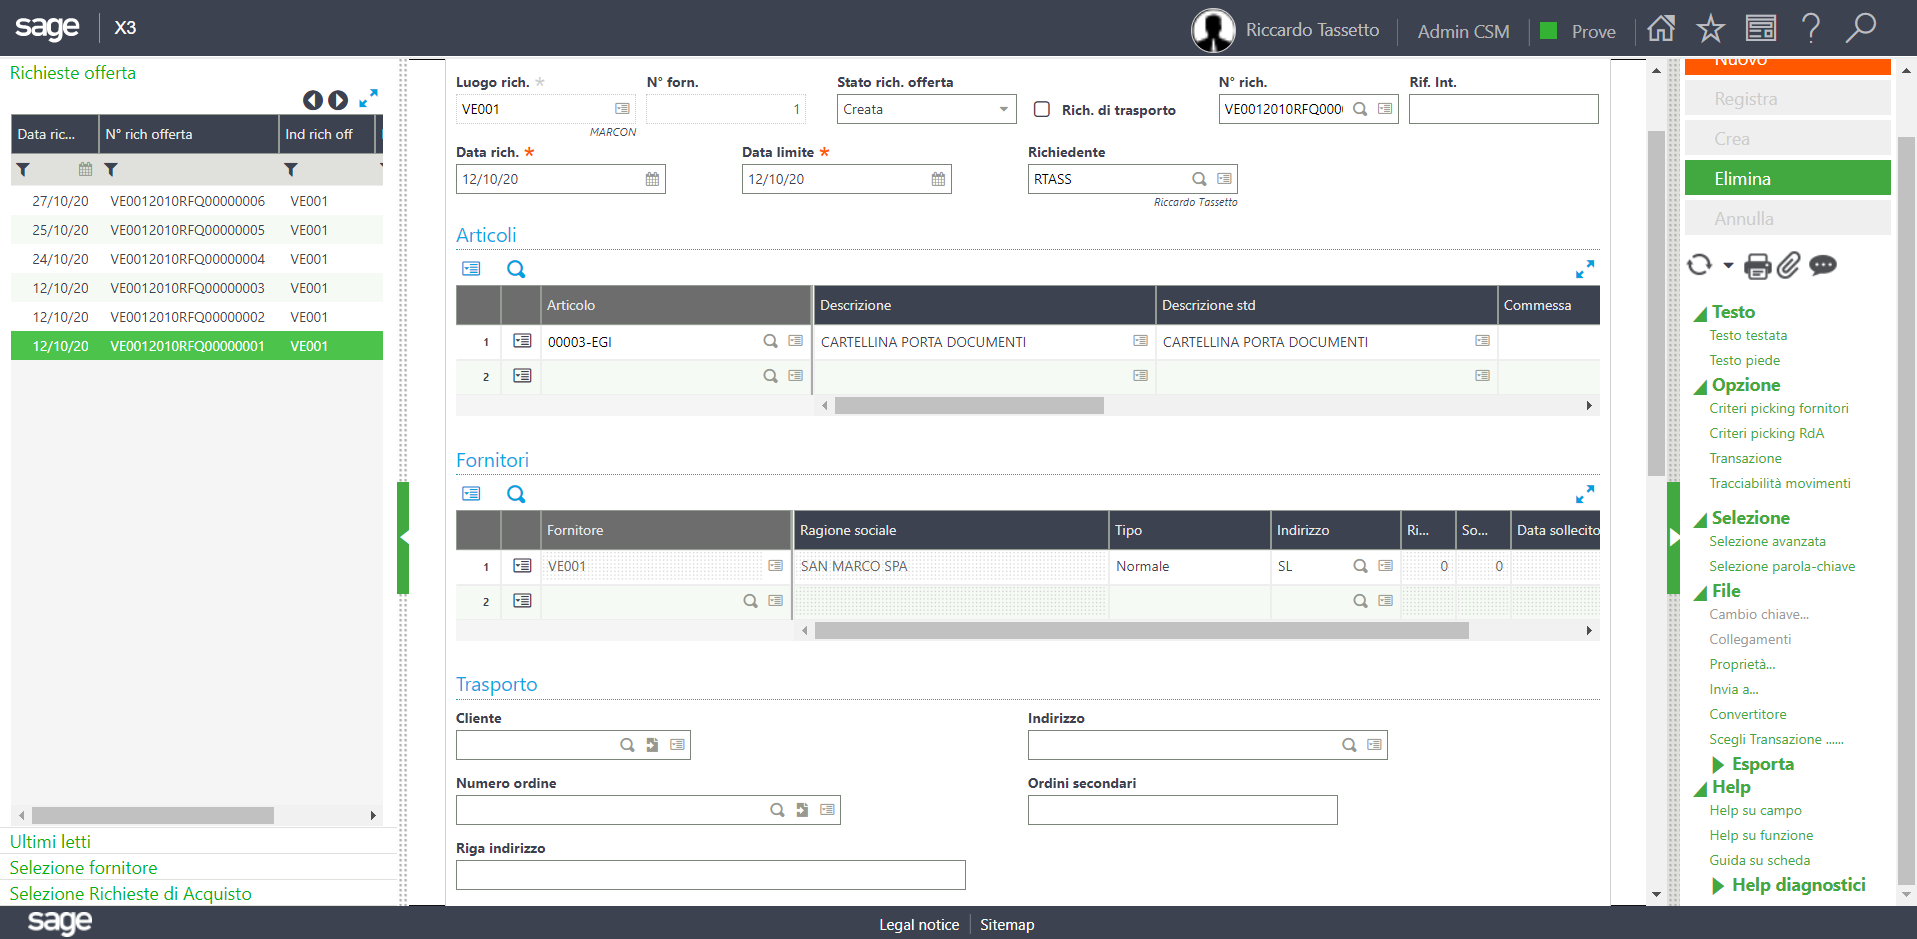
\includegraphics[height=6cm]{videata-x3}
		\caption{Schermata che mostra la rappresentazione di una richiesta di offerta.}
	\end{center}
\end{figure}


\subsubsection{Personalizzazione dell'oggetto X3}
Attraverso la documentazione presente, ho individuato quali tabelle del database erano state utilizzate per generare l'oggetto X3 che gestiva le richieste di offerta.
A quel punto ho potuto, tramite il dizionario delle tabelle presente nell'interfaccia web, aggiungere i campi necessari alla gestione delle richieste, individuati durante l'analisi con i \textit{key users}.
Per poter riuscire a gestire i due tipi di richieste di offerta, che ricordo essere richiesta di beni materiali e richiesta di trasporto, tramite un unico oggetto X3 ho sfruttato una funzione chiamata \textbf{transazione di inserimento}.
Questa permette di gestire le parametrizzazioni per la personalizzazione delle videate di inserimento delle richieste d'offerta.
Viene inizializzata all'installazione del software una transazione standard di inserimento per ogni oggetto X3. 
Nel mio caso ho agito in questo modo:
\begin{itemize}
	\item ho utilizzato la transazione standard (\textit{STD}) per personalizzare la videata di inserimento della richiesta di beni materiali;
	\item ho creato una nuova transazione (\textit{ALL}) e l'ho utilizzata per personalizzare la videata di inserimento della richiesta di trasporto.
\end{itemize}
In questo modo, ogni volta che si accede alla funzionalità delle richieste di offerta, compare la scelta delle transazione e permette di gestire l'uno o l'altro tipo di richiesta, a seconda della necessità.

\begin{figure}[htbp]
	\begin{center}
		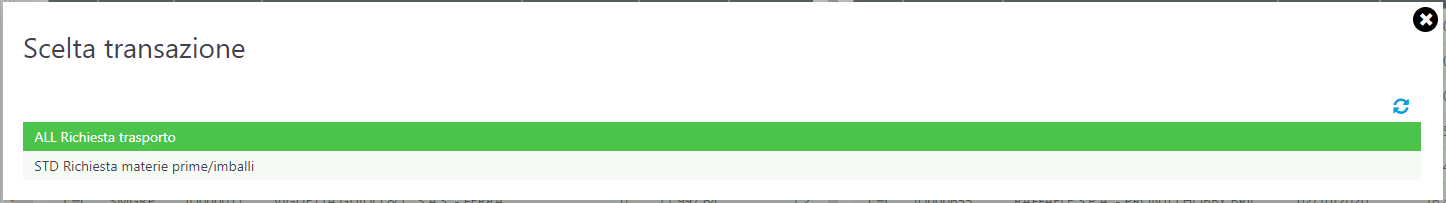
\includegraphics[height=1.8cm]{transazione-x3}
		\caption{Schermata che mostra la scelta della transazione all'apertura delle richieste di offerta.}
	\end{center}
\end{figure}

\subsubsection{Progettazione dell'interfaccia}
L'interfaccia all'interno di Sage X3 è stata progettata con il designer web del gestionale.
Una volta aggiunti i campi necessari all'oggetto, è possibile personalizzare l'interfaccia attraverso:
\begin{itemize}
	\item \textit{drag and drop} degli elementi presenti a video;
	\item  selezione di un elemento a video e utilizzo di una delle operazioni disponibili sul menù di destra, che operano sulla formattazione e visibilità degli elementi.
\end{itemize}
L'impostazione data all'interfaccia è stata resa il più possibile simile al modulo cartaceo utilizzato, dividendola in sezioni corrispondenti ai vari uffici competenti.

\begin{figure}[htbp]
	\begin{center}
		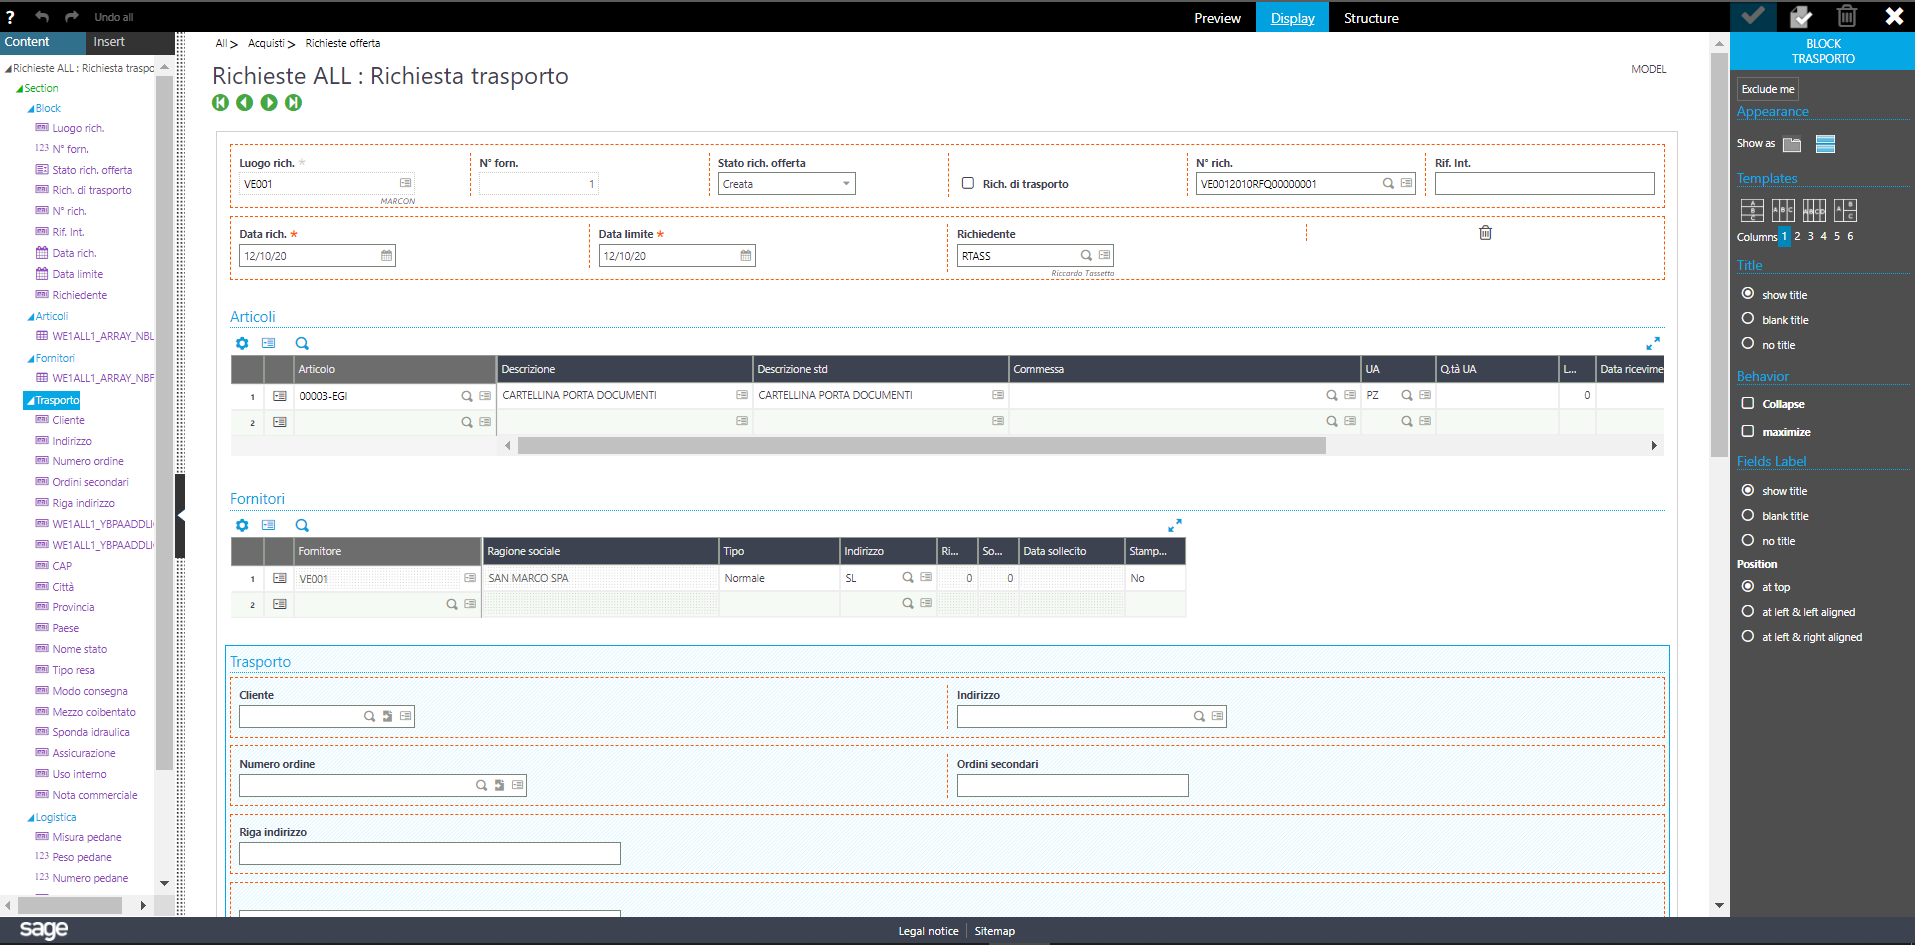
\includegraphics[height=6cm]{designer-x3}
		\caption{Schermata che mostra il designer web di X3.}
	\end{center}
\end{figure}

\subsubsection{Funzionamento}
Alla creazione di una richiesta di offerta, sia essa di acquisto beni materiali o di trasporto, all'interno di una delle tabelle del database che definisce l'oggetto X3 viene creato automaticamente un id chiamato \textit{AUUID} che associa univocamente ogni fornitore coinvolto con la relativa richiesta di offerta.
Una volta compilata nei relativi campi dagli utenti coinvolti, attraverso la funzionalità presente in Sage X3 di invio e-mail, viene spedita una e-mail ad ogni fornitore contenente il corrispondente \textit{AUUID}, che utilizzeranno come \textit{token} al momento dell'autenticazione nell'applicazione web.

%**************************************************************

\subsection{Web Services}
Dopo la formazione sulla tecnologia non ancora affrontata, ho creato i servizi
necessari alla comunicazione bidirezionale tra webapp e gestionale.

\subsubsection{Web services in X3}
L'applicazione web comunica con la base di dati del gestionale tramite \textit{web service SOAP}.
Un \textit{web service SOAP} offre una lista di metodi che possono essere invocati da applicazioni client per svolgere una determinata funzionalità.
Ogni \textit{web service} è legato ad un \textit{dossier} X3. Un \textit{dossier} è una singola ed univoca installazione X3 che ha a disposizione:
\begin{itemize}
	\item una piattaforma tecnologica (runtime server, database server, web server ecc);
	\item un numero di \textit{folder} con organizzazione gerarchica;
	\item \textit{directories} sull'\textit{application server}.
\end{itemize}
Un \textit{dossier} è identificato da un nome e un codice definiti sulla console web.
Lo stesso \textit{web service} può essere definito su più \textit{dossier}.


\begin{figure}[htbp]
	\begin{center}
		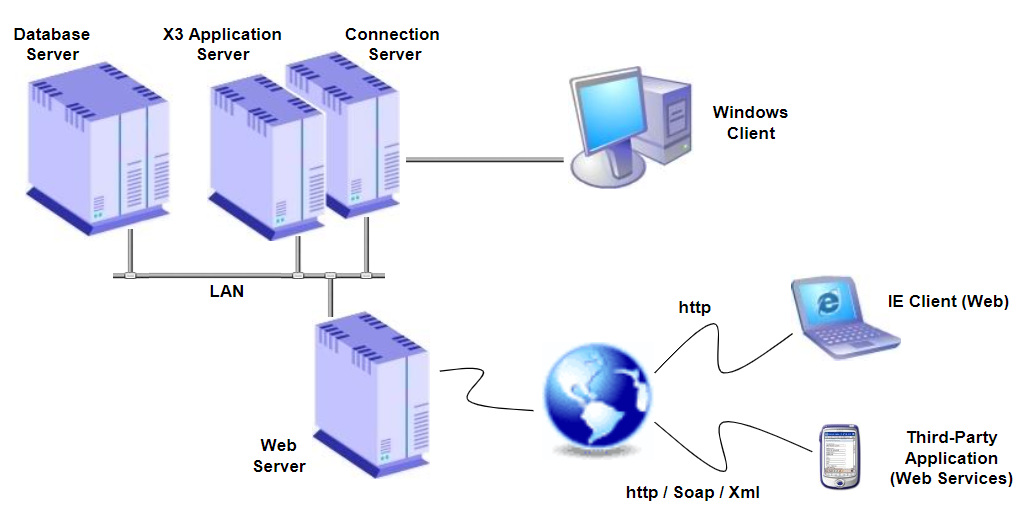
\includegraphics[height=6cm]{architettura-x3}
		\caption{Rappresentazione grafica dell'architettura di una installazione di Sage X3.\newline \textbf{Fonte:} Documentazione Online Help Center di Sage X3}
	\end{center}
\end{figure}




All'interno di Sage X3 è presente una \textit{utility} che permette la pubblicazione di un \textit{web service}: una semplice funzione che trasforma un sottoprogramma o un oggetto X3 in un \textit{web service} con un nome pubblico.
Nel mio caso, ho utilizzato questa \textit{utility} per pubblicare due \textit{web service}, che fornissero i metodi di lettura, modifica e scrittura dell'oggetto X3 corrispondente alla richiesta di offerta, rispettivamente:
\begin{itemize}
	\item 1 \textit{web service}, chiamato \textit{WSYPQHSTD}, che offre i metodi per la richiesta di offerta di beni materiali (generata dalla transazione \textit{STD}); 
	\item 1 \textit{web service}, chiamato \textit{WSYPQHALL}, che offre i metodi per la richiesta di offerta di trasporto (generata dalla transazione \textit{ALL}).
\end{itemize}


\begin{figure}[htbp]
	\begin{center}
		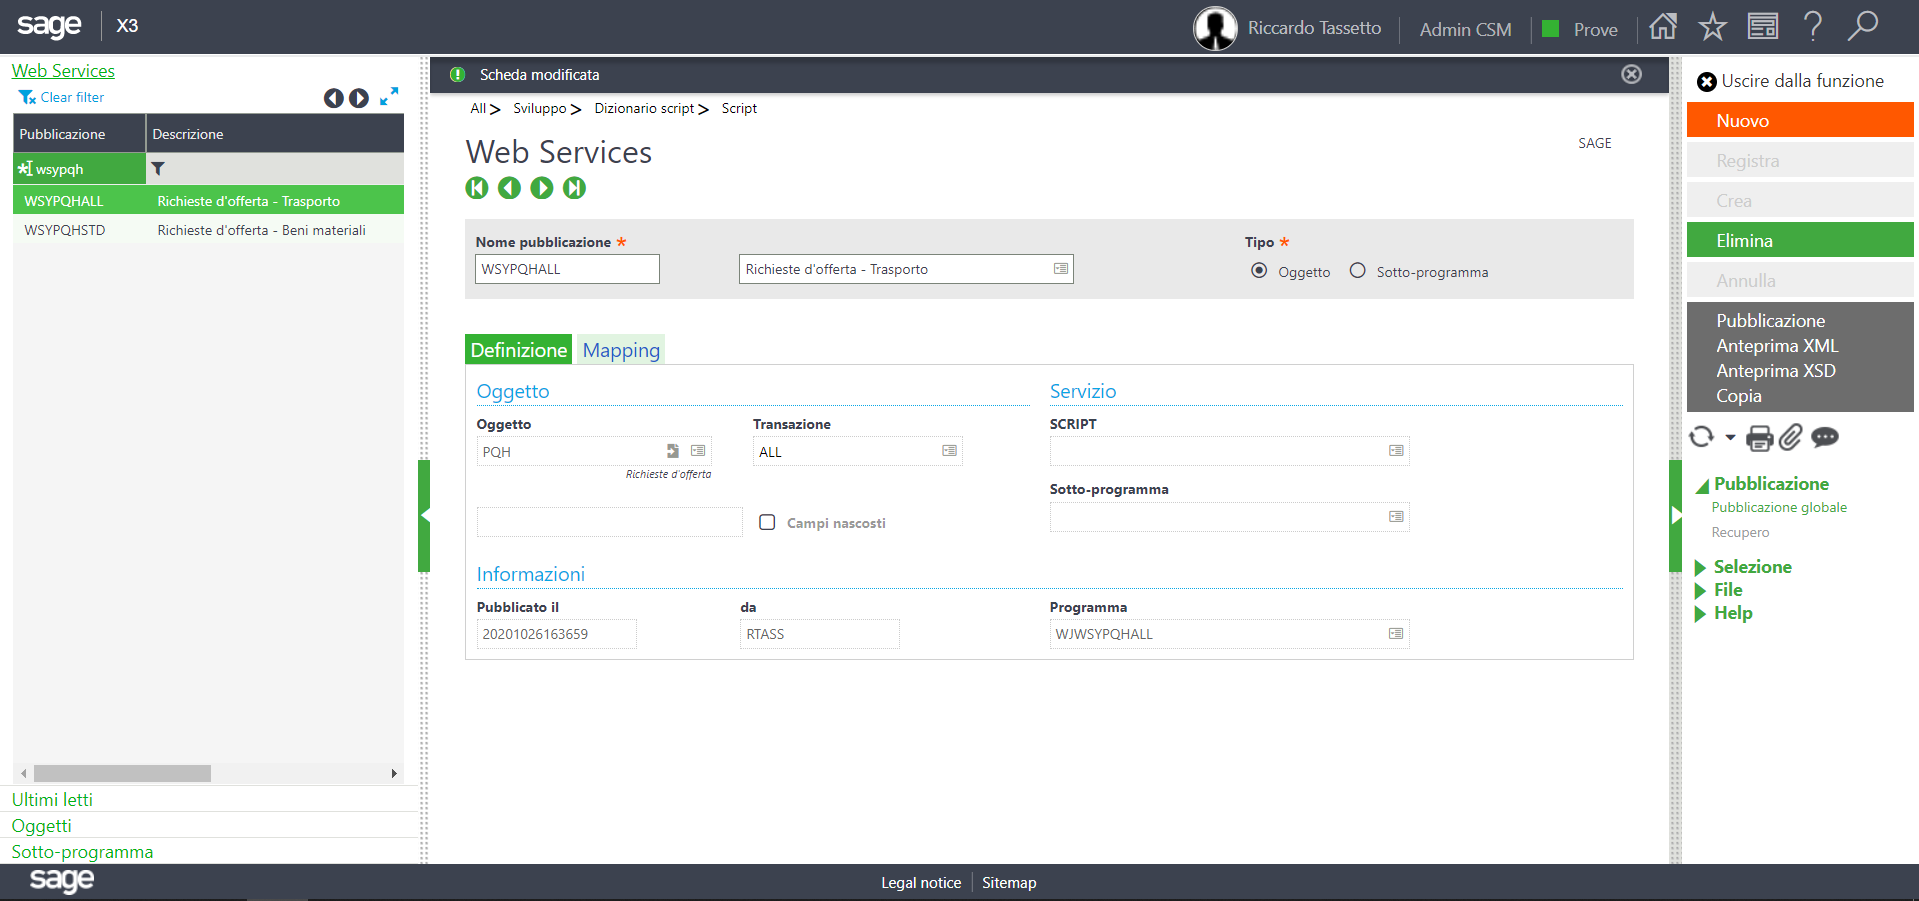
\includegraphics[height=6cm]{creazione-ws-x3}
		\caption{Schermata che mostra i web service creati.}
	\end{center}
\end{figure}

Oltre a questi, ho creato un ulteriore web service, chiamato \textit{WSYPQHAUTH}, personalizzando una routine già presente nel software. 
Questo servizio viene utilizzato in fase di autenticazione del fornitore all'interno dell'applicazione web. 
Permette infatti, dato il \textit{token} chiamato \textit{AUUID} inserito dal fornitore, di recuperare il codice univoco della richiesta di offerta a cui è legato, permettendo quindi all'applicazione web di recuperare i dati dell'offerta tramite i \textit{web service} \textit{WSYPQHSTD} e \textit{WSYPQHALL} descritti in precedenza.

\subsubsection{Gestione della risposta}
Per poter gestire le risposte ricevute dai fornitori, ho creato un web service sull'oggetto X3 di risposta alle richieste di offerta (\textit{PPD} chiamato \textit{WSYPPD}.
Permette infatti, una volta che il fornitore invia la sua risposta tramite l'applicazione web, di creare una nuova istanza dell'oggetto \textit{PPD} contenente i dati inseriti nella risposta. Oltre a questo, l'oggetto contiene anche un riferimento alla richiesta di offerta a cui è associato, in questo modo il software gestionale riesce in autonomia a collegare i due oggetti e permettere all'utente aziendale di visualizzarla. 
%**************************************************************


\subsection{Applicazione web}
Il design pattern utilizzato per la realizzazione dell'applicazione web è l'\textit{MVC}.
Questa tecnica di programmazione separa l'applicazione in tre parti:
\begin{itemize}
	\item \textbf{Model}, che fornisce i metodi per accedere ai dati;
	\item \textbf{View}, che visualizza i dati contenuti nel \textit{model} e permette l'interazione all'utente;
	\item \textbf{Controller}, che si occupa di ricevere gli input dall'utente (attaverso la \textit{view}) e li attua agendo sui dati contenuti nel \textit{model}.
\end{itemize}

\begin{figure}[htbp]
	\begin{center}
		
\includegraphics[height=6cm]{login-webapp}
		\caption{Schermata di autenticazione della webapp.}
	\end{center}
\end{figure}

\subsubsection{Connessione ad X3}
Per poter utilizzare i web service SOAP nella mia applicazione web, è stato necessario creare una \textit{web reference}, ovvero un riferimento ad un insieme di servizi web.
Grazie al \textit{tool} messo a disposizione da Visual Studio, ho potuto aggiungere il \textit{WSDL} di Sage X3, ovvero un documento \textit{XML} che descrive come interagire con il servizio in questione, che contiene:
\begin{itemize}
	\item le operazioni che il servizio mette a disposizione;
	\item il protocollo di comunicazione da utilizzare per accedere al servizio;
	\item il formato dei messaggi accettati in input;
	\item il formato dei messaggi restituiti e il loro output;
	\item gli endpoint di ogni funzione.
\end{itemize}
A questo punto, con i metodi eredidati dal \textit{WSDL}, è possibile implementare una funzione di autenticazione, che andrà successivamente aggiunta all'interno dell'\textit{header} della richieste \textit{SOAP}.


%\subsubsection{Utilizzo di JQuery}

\subsubsection{Funzionamento}
Il fornitore si collega all'applicazione web, dove inserisce nella schermata di autenticazione il \textit{token} ricevuto via e-mail.
Ad autenticazione riuscita, viene caricato il form della richiesta a lui inviata, permettendogli di vedere in dettaglio le informazioni necessarie.
Se dovesse scegliere di inviare una risposta, dopo aver compilato i campi necessari ha la possibilità di inviarla cliccando sul tasto conferma; a questo punto viene creato un oggetto di risposta \textit{PPD} contenente i dati inseriti nel \textit{form} e il riferimento alla richiesta di offerta associata.
Se invece il fornitore intende rifiutare la richiesta, tramite il pulsante di rifiuto viene inviata una comunicazione che notifica l'utente aziendale di riferimento.

\begin{figure}[htbp]
	\begin{center}
		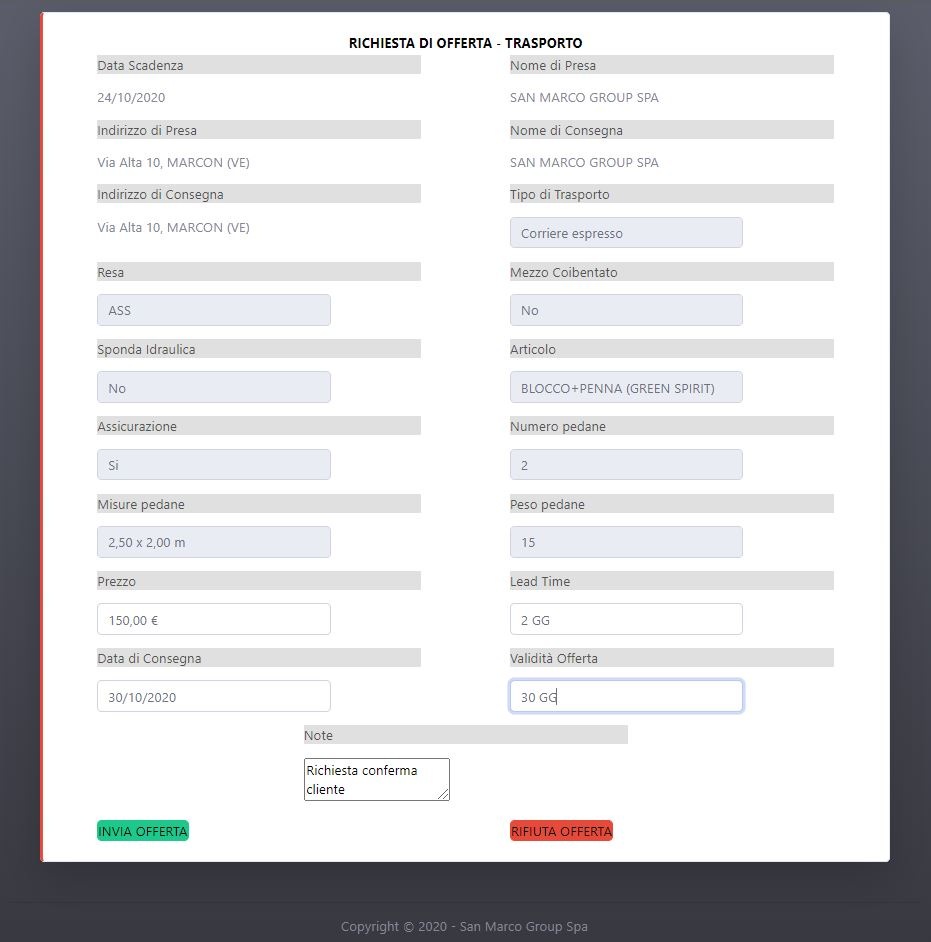
\includegraphics[height=9cm]{form-webapp}
		\caption{Form di inserimento della \textit{webapp} di una risposta a una richiesta di trasporto.}
	\end{center}
\end{figure}
%**************************************************************

\newpage 
\subsection{Reportistica}
Dopo la formazione sullo strumento per la produzione di stampe \textit{Crystal Report}, ho creato il dettaglio della richiesta di offerta.
Attraverso il \textit{tool} disponibile sullo strumento, è possibile collegarsi all'origine dati scelta.
Ho sfruttato il \textit{template} disponibile in Sage X3 della bolla di richiesta offerta e personalizzato il report seguendo il modello dell'attuale cartaceo utilizzato.
Per poter inserire i valori dei campi non ancora presenti sul report, è stato sufficiente selezionarli dalle tabelle del database collegate.

\subsubsection{Report BI}
Dopo un'analisi con il Purchase Manager e con il supporto del tutor aziendale, ho identificato dei dati interessanti al fine di migliorare il processo.
La soluzione proposta permette di tracciare la richiesta dalla sua creazione fino alla risposta dei fornitori. In questo modo è possibile raccogliere una serie di informazioni utili all'ufficio Acquisti che, con le numerose operazioni svolte extra sistema nella precedente gestione, erano difficilmente tracciabili:
\begin{itemize}
	\item \textbf{numero delle richieste di trasporto/numero delle richieste accettate dal cliente}, diventa essenziale individuare quante delle richieste di trasporto che partono dall'ufficio Acquisti e superano la gara dei fornitori, vengono effettivamente accettate dal cliente che richiede il trasporto;
	\item \textbf{numero dei fornitori che rispondono alla richiesta}, altro dato che può essere utilizzato nel metodo di valutazione dell'affidabilità di un fornitore;
	\item \textbf{numero delle richieste di trasporto ad uso interno}, molte richieste vengono fatte con lo scopo di avere una quotazione per un servizio di trasporto e non vengono proposte al cliente finale. Grazie al campo selezionabile all'interno dell'interfaccia utente in Sage X3  al momento della creazione, è possibile conoscere il numero di queste richieste che andranno considerate diversamente dalle richieste con fine di vendita di un servizio;
	\item \textbf{data proposta/data bolla}, confrontando la data proposta di consegna del materiale acquistato con la data della bolla del trasportatore, che corrisponde quindi all'effettiva consegna della merce, si ha modo di utilizzare questo dato nella valutazione dell'affidabilità del fornitore.
\end{itemize}



%**************************************************************


\section{Verifica e validazione}

\subsection{Verifica}
La verifica del software è un processo necessario a stabilire che il prodotto e le parti che lo compongono, risponda ai requisiti fissati in precedenza.
In un primo momento ho effettuato l'analisi statica, successivamente ho eseguito test di unità e integrazione sugli elementi fondamentali del prodotto.


\paragraph{Analisi statica}
L'analisi statica è una tipologia di analisi del software che non prevede l'esecuzione del codice.
Ho effettuato l'analisi statica più volte durante il periodo di stage, tramite la lettura del codice prodotto nello sviluppo dell'applicazione web, al raggiungimento di ogni punto significativo in termini di codifica.

\paragraph{Test di unità}
Per quanto riguarda l'applicazione web, attraverso il \textit{framework} \textit{MSTest} presente in Visual Studio sono stati eseguiti i test sulle singole unità dell'applicazione web, classi e sui metodi principali che compongono il progetto.\\
Nell'interfaccia del gestionale invece, sono stati verificato il funzionamento dei campi, in particolare sui tipi di dato accettati e il funzionamento delle operazioni di creazione, modifica ed eliminazione delle richieste di offerta.

\paragraph{Test di integrazione}
Essendo ancora in corso lo sviluppo del gestionale, non è stato possibile effettuare test sotto stress o che verificassero il funzionamento di funzionalità come l'invio automatico del \textit{token} al fornitore. Sono stati quindi fatti dei test ad hoc per verificare il funzionamento delle funzionalità.\\
Nonostante questo, dopo una valutazione con il tutor aziendale siamo arrivati alla conclusione che il lavoro fatto risulta comunque sufficiente.
I \textit{web service} sono stati testati attraverso il tester di Sage X3. Questo \textit{tool} permette, inserendo i parametri di configurazione, la verifica dei metodi principali disponibili (lettura, modifica, salvataggio, ecc.) sui \textit{web service} pubblicati.


\begin{figure}[htbp]
	\begin{center}
		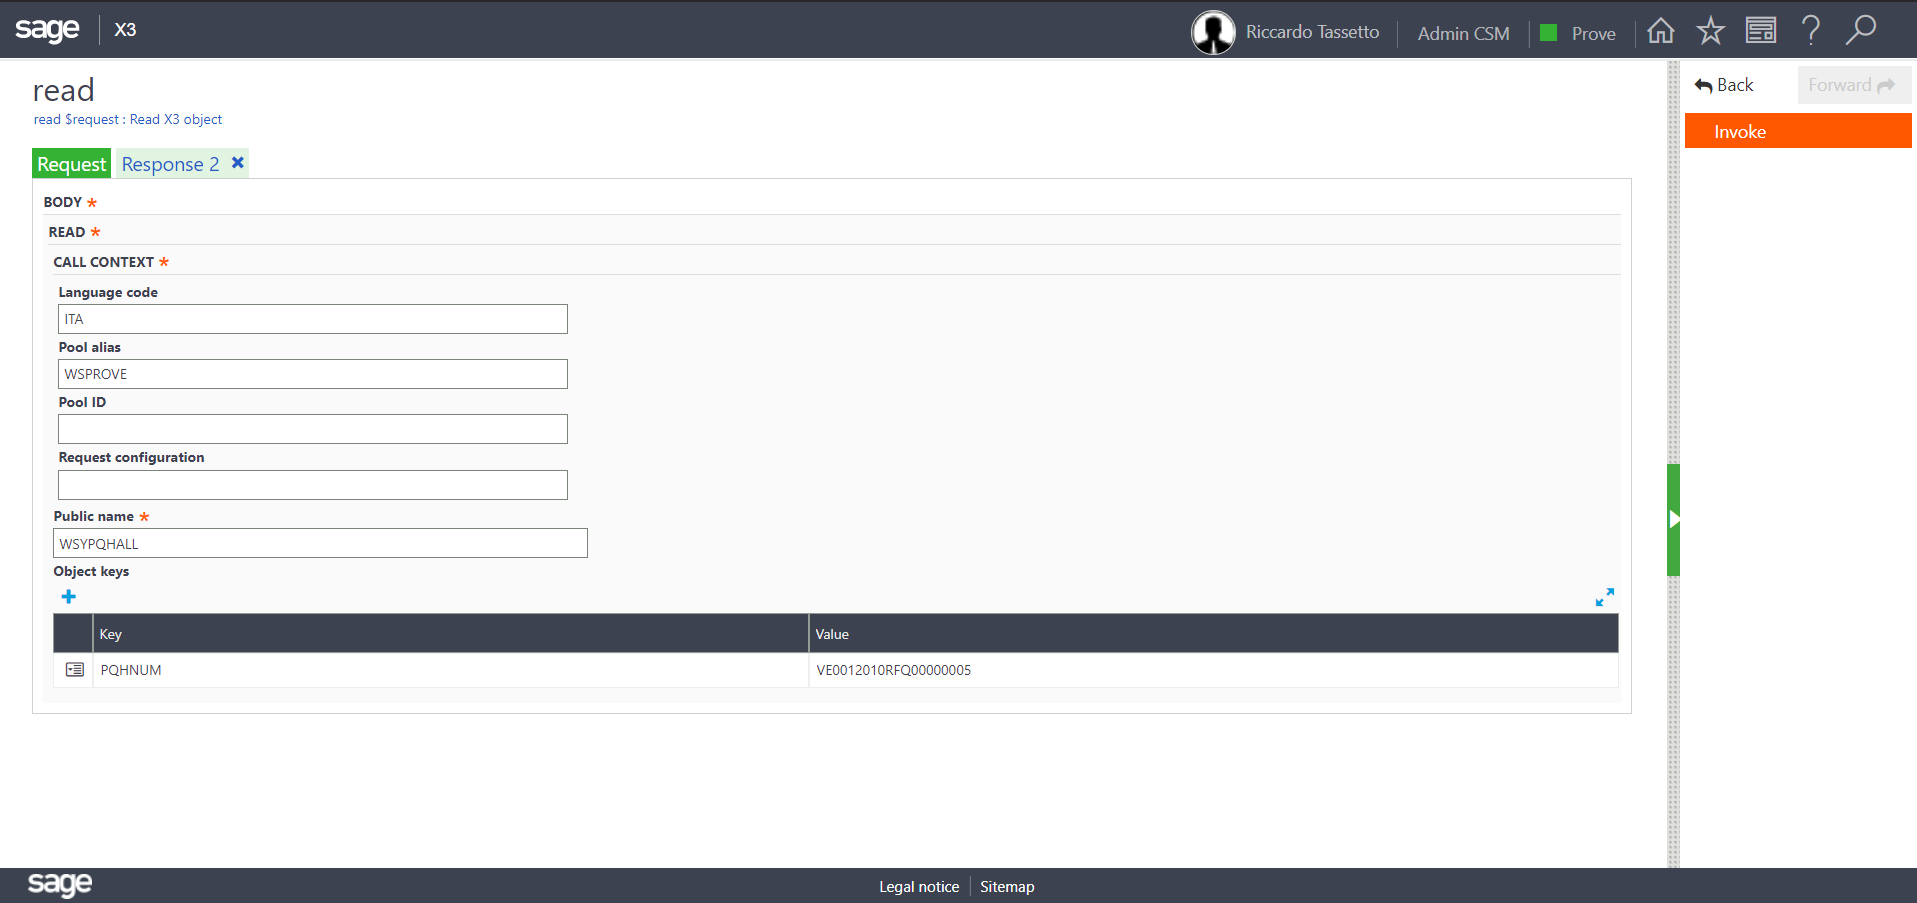
\includegraphics[height=6cm]{ws-tester-request}
		\caption{Schermata che mostra una richiesta dal web service tester di Sage X3.}
	\end{center}
\end{figure}

\begin{figure}[htbp]
	\begin{center}
		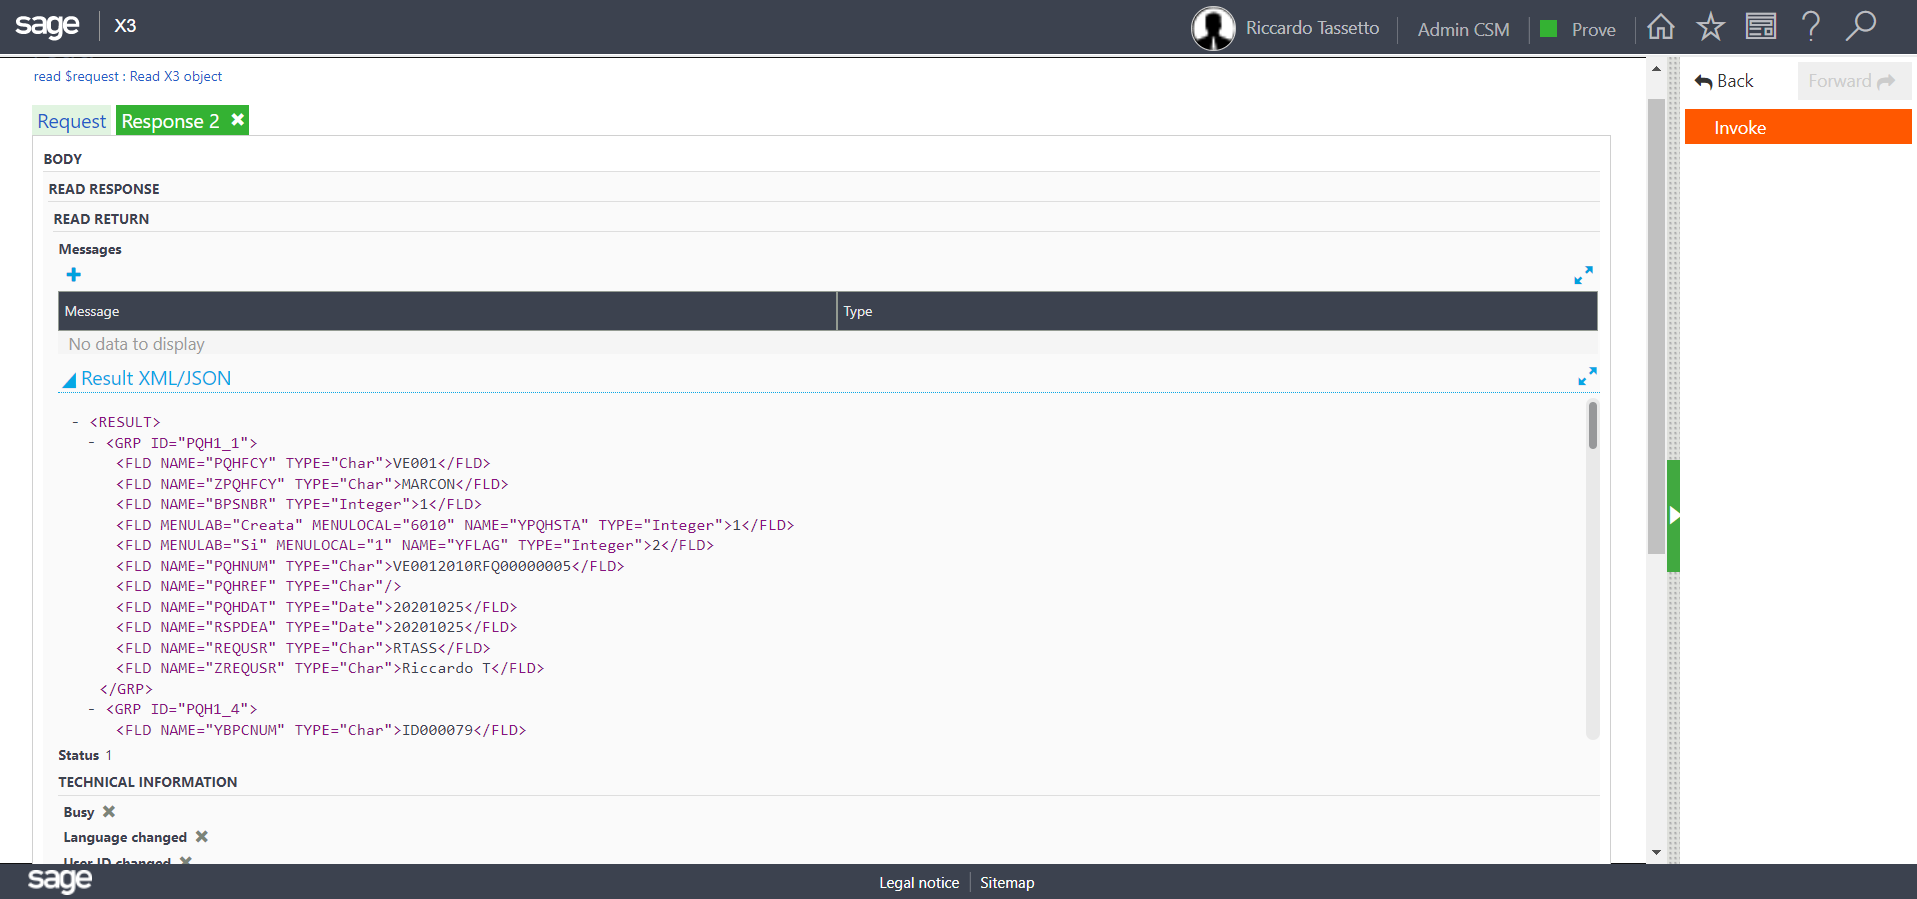
\includegraphics[height=6cm]{ws-tester-response}
		\caption{Schermata che mostra una risposta dal web service tester di Sage X3.}
	\end{center}
\end{figure}

\newpage
\subsection{Validazione}
Il processo di validazione del software è un controllo che permette di accertare se il prodotto finale corrisponde alle attese e risulta quindi conforme ai requisiti dichiarati inizialmente.
Al termine dello stage ho effettuato autonomamente una validazione interna verificando il funzionamento dell'interfaccia sviluppata in Sage X3 e svolgendo i test sulle funzionalità implementate nell'applicazione web, simulando rispettivamente l'uso da parte di un utente aziendale e l'uso da parte di un fornitore.
Essendo ancora in corso lo sviluppo del nuovo gestionale e di tutte le funzionalità previste, ho mostrato il prodotto ed il suo funzionamento al tutor aziendale che ha valutato positivamente il lavoro.

%**************************************************************


\section{Consuntivo finale}

\subsection{Prodotti ottenuti}

I prodotti che ho realizzato, sia documentali che software, richiesti dall'azienda sono i seguenti:

\begin{itemize}
	\item relazione sul processo aziendale coinvolto;
	\item relazione sulla progettazione architetturale;
	\item codice sorgente dell'applicazione web;
	\item interfaccia personalizzata sul gestionale;
	\item manuale e documentazione riguardante la struttura dell'applicazione web per
	manutenzione ed eventuali integrazioni;
	\item report di dettaglio e di analisi \textit{BI}.
\end{itemize}

%**************************************************************

\subsection{Copertura di requisiti e test}

Tutti i requisiti delineati durante la fase di analisi sia relativi all'applicazione web che all'interfaccia del gestionale sono stati raggiunti.

\begin{center}
	\begin{longtable}{ | c| c | c|}
		\caption{Tabella di riepilogo requisiti soddisfatti.}\\		
		\hline
		\textbf{Tipo} & \textbf{Soddisfatti} & \textbf{Non soddisfatti} \\
		\hline
		\textbf{Funzionale} & 26 & 0 \\
		\hline
		\textbf{Qualitativo} & 1 & 0 \\
		\hline
		\textbf{Vincolo} & 3 & 0 \\
		\hline
		\textbf{Prestazionale} & 0 & 0 \\
		\hline
		\textbf{Totale} & 30 & 0 \\
		\hline
	\end{longtable}
\end{center}

Nonostante il suo raggiungimento, non mi ritengo completamente soddisfatto del risultato relativo al requisito desiderabile. Era infatti mio desiderio approfondire maggiormente l'analisi dei dati con i soggetti interessati e capire in che modo possono essere usati per stimolare il cambiamento ed eliminare le inefficienze.
Questo è dovuto alla mancanza di tempo data dal prolungarsi dell'attività di verifica dei web service, che hanno richiesto più tempo del previsto sia per la difficoltà personale che ho trovato nell'affrontare la tecnologia sconosciuta, che per alcuni problemi esterni all'azienda che hanno portato ad un rilascio posticipato del certificato digitale \textit{SSL} per il server web di Sage X3.
Per quanto concerne la copertura dei test, non era stata richiesta una soglia minima di \textit{Code Coverage}. Per l'applicazione web, i test effettuati fatti sui metodi principali raggiungono il 70\% di \textit{Code Coverage}, risultato considerato sufficiente dal tutor aziendale.
I web service, come descritto in 3.4.1, sono stati testati attraverso il modulo integrato in Sage X3.

%**************************************************************

%**************************************************************

%\section{Analisi preventiva dei rischi}

%Durante la fase di analisi iniziale sono stati individuati alcuni possibili rischi a cui si potrà andare incontro.
%Si è quindi proceduto a elaborare delle possibili soluzioni per far fronte a tali rischi.\\

%\begin{risk}{Performance del simulatore hardware}
%    \riskdescription{le performance del simulatore hardware e la comunicazione con questo potrebbero risultare lenti o non abbastanza buoni da causare il fallimento dei test}
%    \risksolution{coinvolgimento del responsabile a capo del progetto relativo il simulatore hardware}
 %   \label{risk:hardware-simulator} 
%\end{risk}

